\documentclass{article}
\setlength{\parskip}{5pt} % esp. entre parrafos
\setlength{\parindent}{0pt} % esp. al inicio de un parrafo
\usepackage{listings} % listings
\usepackage{color} %colores
\usepackage{amsmath} % mates
\usepackage[sort&compress,numbers]{natbib} % referencias
\usepackage{url} % que las URLs se vean lindos
\usepackage[top=15mm,left=20mm,right=20mm,bottom=25mm]{geometry} % margenes
\usepackage{hyperref} % ligas de URLs
\usepackage{graphicx} % poner figuras
\usepackage[spanish]{babel} % otros idiomas

\author{Claudia Lizeth Hern\'andez Ram\'irez} % author
\title{Homework 4 - Diagrama Voronoi.} % titulo
\date{\today}

\definecolor{mypink}{rgb}{0.976, 0.462, 0.847}
\definecolor{mygray}{rgb}{0.976, 0.980, 0.980}
\definecolor{myblue}{rgb}{0.258, 0.682, 1}
\definecolor{mypink2}{rgb}{0.525, 0.054, 0.4}
\lstset{ 
  backgroundcolor=\color{mygray},
  commentstyle=\color{myblue},
  keywordstyle=\color{mypink}, 
  numberstyle=\tiny\color{mypink}
  stringstyle=\color{mypink2}, 
  breaklines=true,
}


\begin{document} % inicia contenido

\maketitle % cabecera

% RESUMEEEEEEEEEEEEEEEN
\begin{abstract} % resumen
  \centering
Las diferencias entre las medianas no son estad\'{i}sticamente significativas.
  
\end{abstract}


% INTRODUCCIOOOOOOOOOOOON
\section{Introducci\'{o}n}\label{intro} % seccion y etiqueta
Examina el efecto del n\'umero de semillas , manteniendo constante el tamaño de la zona , en la penetraci\'on de las grietas que se forman en t\'erminos de la mayor distancia Manhattan entre la grieta y el exterior de la pieza, visualizando los resultados con diagramas caja-bigote o similar sobre las r\'eplicas y aplicando m\'etodos estad\'isticos para establecer el efecto tiene, si es que tenga,  en ello.



% DESARROLLOOOOOOOOOOOO
\section{Desarrollo}\label{desarrollo} % Desarrollo de la tarea

Comenzamos utilizando el c\'odigo proporcionado en clase por la Dra Elisa\citep{CodigoBase}.
Se modific\'o el n\'umero de semillas agregando un ciclo \texttt{FOR}.
\begin{lstlisting} [language=R, caption= Fragmento de c\'odigo para variar el n\'umero de semillas.]

datos = data.frame()
n <-  15
for (k in c(10, 20, 30)) {
zona <- matrix(rep(0, n * n), nrow = n, ncol = n)
x <- rep(0, k) # ocupamos almacenar las coordenadas x de las semillas
y <- rep(0, k) # igual como las coordenadas y de las semillas

for (semilla in 1:k) {
  while (TRUE) { # hasta que hallamos una posicion vacia para la semilla
    fila <- sample(1:n, 1)
    columna <- sample(1:n, 1)
    if (zona[fila, columna] == 0) {
      zona[fila, columna] = semilla
      x[semilla] <- columna
      y[semilla] <- fila
      break
      }
    }
  }
}
\end{lstlisting}

Posteriormente, gener\'e una matriz que dejaba ver las \'areas de \texttt{grieta} la cual export\'e a un archivo \texttt{.xlsx}.
\newpage

\begin{lstlisting} [language=R, caption= Fragmento de c\'odigo que genera matriz de grieta.]

if (largo >= limite) {
    png(paste("p4g_", replica, ".png", sep=""))
    par(mar = c(0,0,0,0))
    image(rotate(grieta), col=rainbow(k+1), xaxt='n', yaxt='n')
    graphics.off()
  }
  return(grieta)
}
suppressMessages(library(doParallel))
registerDoParallel(makeCluster(detectCores() - 2))
manhattanmatriz <- foreach(r = 1:1, .combine=c) %dopar% propaga(r)
stopImplicitCluster()
manhattanmatriz
datos = rbind(datos, manhattanmatriz)
write_xlsx(datos, "midataframe3015.xlsx") #exporta a xlsx

\end{lstlisting}

Una vez exportados, obtuve los valores m\'aximos de distancia Manhattan entre la grieta y el exterior de mi pieza;
\begin{table}[ht]
    \centering
    \caption{Valores de distancia mayor Manhattan entre grieta y exterior de pieza.}
    \begin{tabular}{|c|c|c|c|}
    \hline
    Iteraci\'on & N\'umero de semillas & & \\
    \hline
   '' & 10 & 20 & 30 \\
    \hline
    1 & 8 & 8 & 8 \\
    \hline
    2 & 5 & 4 & 5 \\
    \hline
    3 & 7 & 7 & 6 \\
    \hline
    4 & 4 & 5 & 7 \\
    \hline
    5 & 8 & 7 & 5 \\
    \hline
    6 & 7 & 8 & 7 \\
    \hline
    7 & 5 & 7 & 4 \\
    \hline
    8 & 3 & 7 & 7 \\
    \hline
    9 & 6 & 4 & 8 \\
    \hline
    10 & 4 & 4 & 8 \\
    \hline
    11 & 8 & 7 & 7 \\
    \hline
    12 & 8 & 5 & 7 \\
    \hline
    13 & 7 & 8 & 7 \\
    \hline
    14 & 7 & 6 & 5 \\
    \hline
    15 & 7 & 8 & 7 \\
    \hline
    \end{tabular}
    \label{cuadro 1}
\end{table}
Mismos que fueron graficados en un \texttt{boxplot}.

\begin{figure}[htbp] % figura
    \centering
    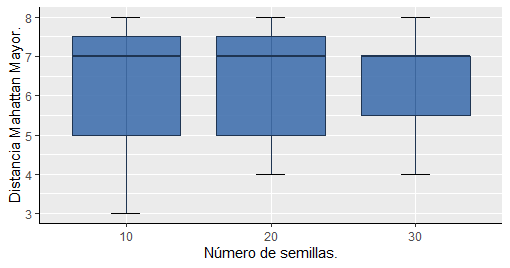
\includegraphics[width=150mm]{Rplot.png} % archivo
    \caption{Distancia mayor Manhattan con variaci\'on en el n\'umero de semillas.}
    \label{Figura 1}
\end{figure}

A simple vista podr\'iamos pensar que estamos tratando con datos que no tienen una distribuci\'on normal, para comprobar esta teor\'ia utilic\'e la prueba de \texttt{shapiro.test}.

\begin{lstlisting} [language=R, caption= Fragmento de c\'odigo utilizado para hacer pruebas de normalidad.]
#pruebas de normalidad Shapiro test

lshap = lapply(datositer, shapiro.test)
lshap[[1]]
lshap = lapply(datositer, shapiro.test)
lshap[[2]]
lshap = lapply(datositer, shapiro.test)
lshap[[3]]
\end{lstlisting}

\begin{table}[ht]
    \centering
    \caption{Resultados obtenidos de prueba de normalidad de Shapiro.} 
    \begin{tabular}{|c|c|c|}
    \hline
    Semilla & W & P  \\
    \hline
    10 & 0.8691 & 0.0327 \\
    \hline
    20 & 0.8433 & 0.0.140 \\
    \hline
    30 & 0.850 & 0.0204\\
    \hline
\end{tabular}
    \label{cuadro 2}
\end{table}
\newpage

Como es evidente, se rechaza hip\'otesis nula y podemos confirmar que nuestros datos no tienen una distribución normal, por lo que preocedemos a utilizar una prueba no param\'etrica, como lo es \texttt{Kruskal Wallis} \cite{SeleccionPruebas, InterpretacionKruskalWallis}.


\begin{lstlisting}[language=R, caption= Fragmento de c\'odigo utilizado para hacer pruebas de Kruskal Wallis.]
diez = c(8, 5, 7, 4, 8, 7, 5, 3, 6, 4, 8, 8, 7, 7, 7)
veinte =c(8, 4, 7, 5, 7, 8, 7, 7, 4, 4, 7, 5, 8, 6, 8)
treinta = c(8, 5, 6, 7, 5, 7, 4, 7, 8, 8, 7, 7, 7, 5, 7)
kruskal.test(list(diez, veinte, treinta))
\end{lstlisting}

\begin{table}[ht]
    \centering
    \caption{Resultados obtenidos de prueba Kruskal-Wallis.} 
    \begin{tabular}{|c|c|c|}
    \hline
    Chi cuadrada & DF & P  \\
    \hline
    0.0716 & 2 & 0.0.9648 \\
    \hline
\end{tabular}
    \label{cuadro 3}
\end{table}

\newpage

%CONCLUSIOOOON
\section{Conclusi\'on}
Teniendo que:

-Hip\'otesis nula: las medias de poblaci\'on son todas iguales.

-Hip\'otesis alternativa: las medias de poblaci\'on no son todas iguales.
y con un nivel de significancia = 0.05 podemos aceptar la hip\'otesis nula, por lo tanto las diferencias entre las medianas no son estad\'isticamente significativas.

% BIBLIOGRAFIAAAAAAS
\bibliography{referencias}
\bibliographystyle{plainnat}
\end{document}


